\documentclass[a0paper,portrait]{baposter}
\usepackage[T1]{fontenc}
\usepackage[scaled]{helvet}
\renewcommand\familydefault{\sfdefault}
\usepackage{graphicx,amsmath,amssymb,array,booktabs,multicol,setspace,url,xcolor}
\usepackage[hidelinks]{hyperref}
\graphicspath{{images/}}
\geometry{tmargin=0mm,bmargin=4mm,lmargin=9mm,rmargin=9mm}
\definecolor{navy}{RGB}{13,71,161} 
\definecolor{ieblue}{RGB}{21,101,192} 
\definecolor{lightblue}{RGB}{25,118,210}
\definecolor{amazonorange}{RGB}{245,124,0}
\definecolor{muted}{RGB}{92,105,126}
\definecolor{softgray}{RGB}{244,246,249}
\definecolor{offwhite}{RGB}{250,249,246}
\newcommand{\titlefont}{\bfseries\Huge\color{offwhite}}
\newcommand{\authorfont}{\bfseries\Large\color{offwhite}}
\newcommand{\headerfont}{\bfseries\large\color{offwhite}}
\newcommand{\smallnote}[1]{{\scriptsize\color{muted}#1}}
\newcommand{\metric}[2]{\begin{minipage}[c]{0.22\linewidth}\centering{\color{navy}\bfseries\LARGE #1}\\[-1mm]{\small #2}\end{minipage}}
\begin{document}
\background{}
\begin{poster}{grid=false,borderColor=offwhite,headerColorOne=ieblue,headerColorTwo=ieblue,headerFontColor=offwhite,boxColorOne=offwhite,headerheight=0mm,boxheaderheight=2.2em,headershape=rectangle,headerfont=\headerfont,textborder=none,headerborder=none,background=plain,bgColorOne=offwhite,boxshade=plain,columns=2}{}{}{}{}
\small

\headerbox{}{name=titlebox,span=2,column=0,row=0,boxheaderheight=0mm,headerColorOne=navy,headerColorTwo=navy,boxColorOne=navy,boxColorTwo=navy}{
\vspace{5mm}\begin{minipage}{0.94\textwidth}
\color{offwhite}\rule{\textwidth}{3pt}\vspace{3mm}
{\titlefont Optimizing Amazon Locker Capacity}\par\vspace{4mm}
{\authorfont YOUR NAME \quad COLLEAGUE NAME}\par\vspace{2mm}
{\large Ship-option capacity reservation under uncertain demand and pickup times}\par
{\small Optimization I \;|\; IE University \;|\; Reproducible Pyomo implementation}
\end{minipage}\vspace{5mm}}

\headerbox{Problem at a glance}{name=overview,span=2,column=0,below=titlebox}{
\begin{minipage}[t]{0.53\linewidth}
\textbf{Decision.} How many requests of each ship option should be accepted at each locker and on each day, while keeping expected occupancy within physical capacity?

\vspace{2mm}The model converts demand forecasts and dwell-time probabilities into expected slot usage. It then maximizes accepted packages across the seven-day planning horizon.
\end{minipage}\hfill
\begin{minipage}[t]{0.43\linewidth}\centering
\metric{4}{lockers}\hfill\metric{7}{days}\hfill\metric{909}{requests}\hfill\metric{88.3\%}{baseline acceptance}
\end{minipage}}

\headerbox{}{name=footer,span=2,column=0,above=bottom,boxheaderheight=0mm,headerColorOne=softgray,headerColorTwo=softgray,boxColorOne=softgray,boxColorTwo=softgray}{
\footnotesize
\textbf{Source and reproducibility.} Numbers and vector figures are generated from this repository's \texttt{data/} and \texttt{reports/} folders. Model context: Sethuraman et al. (2024), ``Amazon Locker Capacity Management,'' \emph{Manufacturing \& Service Operations Management}, doi:10.1287/msom.2021.0544. Poster layout adapted from the open-source ICFO baposter template by Emilio Pisanty.\\
\textbf{Repository:} \url{https://github.com/dloweieu2025-create/amazon-locker-capacity-optimization}}

\headerbox{1. Input data}{name=data,column=0,below=overview}{
\textbf{Demand forecast} $D_{lst}$: requested packages for locker $l$, service $s$, and day $t$. The current instance contains \textbf{909 total requests} across four Madrid lockers.

\vspace{1mm}\textbf{Dwell probability} $q_{sa}$: probability that a package of service $s$ still occupies a slot $a$ days after arrival. Standard shipments remain longer, so they consume more future capacity.

\begin{center}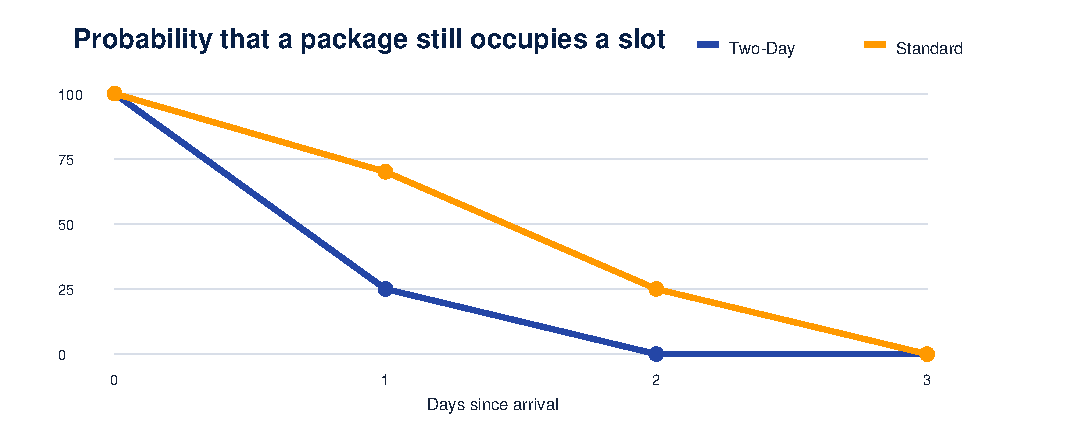
\includegraphics[width=0.84\linewidth]{dwell_probabilities.pdf}\end{center}
\smallnote{Input: \texttt{data/occupancy.csv}. Two-Day: $[1,0.25,0,0]$; Standard: $[1,0.70,0.25,0]$.}}

\headerbox{2. Optimization model}{name=model,column=0,below=data}{
\textbf{Decision variable}
\[x_{lst}\in\mathbb{Z}_{+}: \text{packages accepted at locker }l,\text{ service }s,\text{ day }t.\]
\textbf{Objective}
\[\max \sum_{l\in L}\sum_{s\in S}\sum_{t\in T} x_{lst}.\]
\textbf{Demand bounds}
\[0\le x_{lst}\le D_{lst}\qquad \forall l,s,t.\]
\textbf{Expected-capacity constraints}
\[\sum_{s\in S}\sum_{\tau\le t}q_{s,t-\tau}\,x_{ls\tau}\le C_l\qquad \forall l,t.\]
The resulting formulation is a \textbf{linear integer program}. All coefficients are fixed parameters, and the decision variables are integer counts.}

\headerbox{3. Reproducible workflow}{name=workflow,column=0,below=model}{
\begin{center}
\fcolorbox{ieblue}{lightblue}{\parbox{0.17\linewidth}{\centering\textbf{CSV inputs}\\demand, lockers, dwell}} $\;\Longrightarrow\;$
\fcolorbox{ieblue}{lightblue}{\parbox{0.17\linewidth}{\centering\textbf{Pyomo}\\build MILP}} $\;\Longrightarrow\;$
\fcolorbox{ieblue}{lightblue}{\parbox{0.17\linewidth}{\centering\textbf{HiGHS}\\solve}} $\;\Longrightarrow\;$
\fcolorbox{ieblue}{lightblue}{\parbox{0.17\linewidth}{\centering\textbf{Reports}\\CSV + plots}}
\end{center}
\smallnote{Run \texttt{python src/solve\_capacity.py}. Scenario folders preserve the inputs, solution summaries, and daily occupancy used in this poster.}}

\headerbox{5. Baseline results: 46 slots per locker}{name=baseline,column=1,below=overview}{
\begin{center}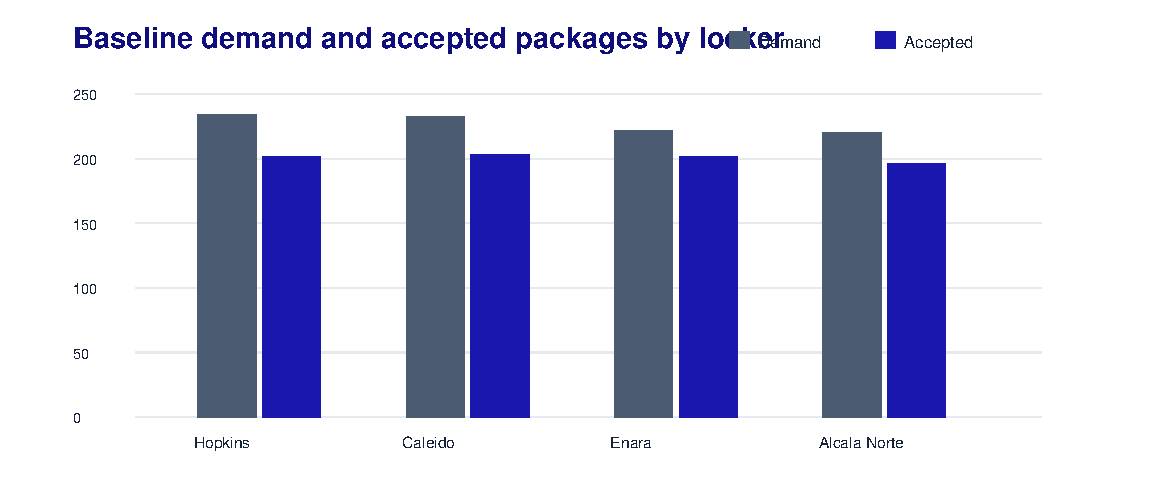
\includegraphics[width=0.88\linewidth]{locker_performance.pdf}\end{center}\vspace{-2mm}
\begin{center}\scriptsize\begin{tabular}{lrrrr}
\toprule
\textbf{Locker} & \textbf{Demand} & \textbf{Accepted} & \textbf{Rejected} & \textbf{Rate}\\
\midrule
Hopkins & 234 & 202 & 32 & 86.3\%\\
Caleido & 233 & 203 & 30 & 87.1\%\\
Enara & 222 & 202 & 20 & 91.0\%\\
Alcala Norte & 220 & 196 & 24 & 89.1\%\\
\midrule
\textbf{Total} & \textbf{909} & \textbf{803} & \textbf{106} & \textbf{88.3\%}\\
\bottomrule
\end{tabular}\end{center}
\begin{center}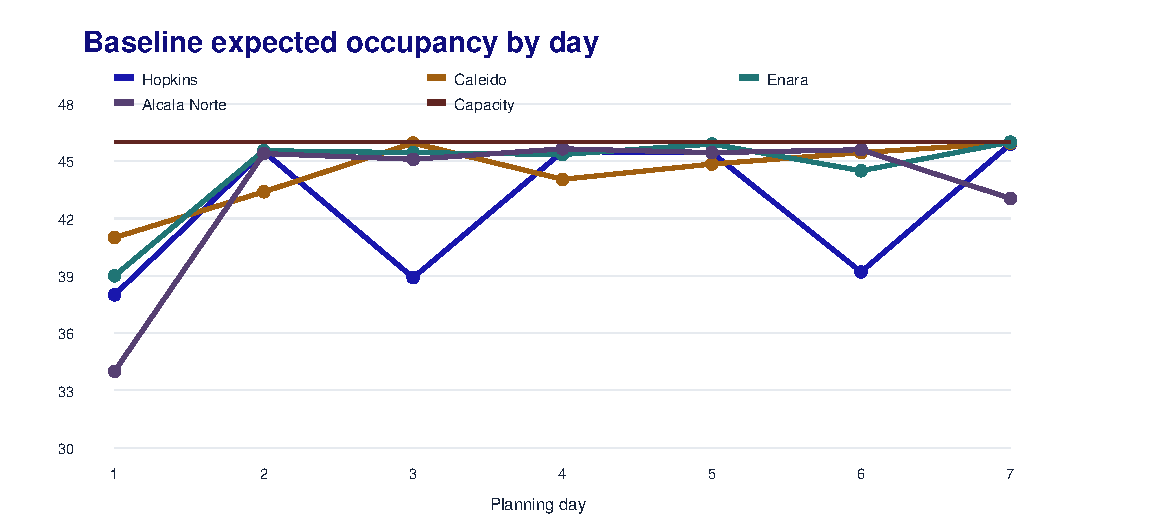
\includegraphics[width=0.88\linewidth]{baseline_occupancy.pdf}\end{center}
\smallnote{Expected occupancy repeatedly approaches the 46-slot limit, showing that capacity---not demand---drives rejections on peak days.}}

\headerbox{6. Scenario analysis}{name=scenarios,column=1,below=baseline}{
\begin{center}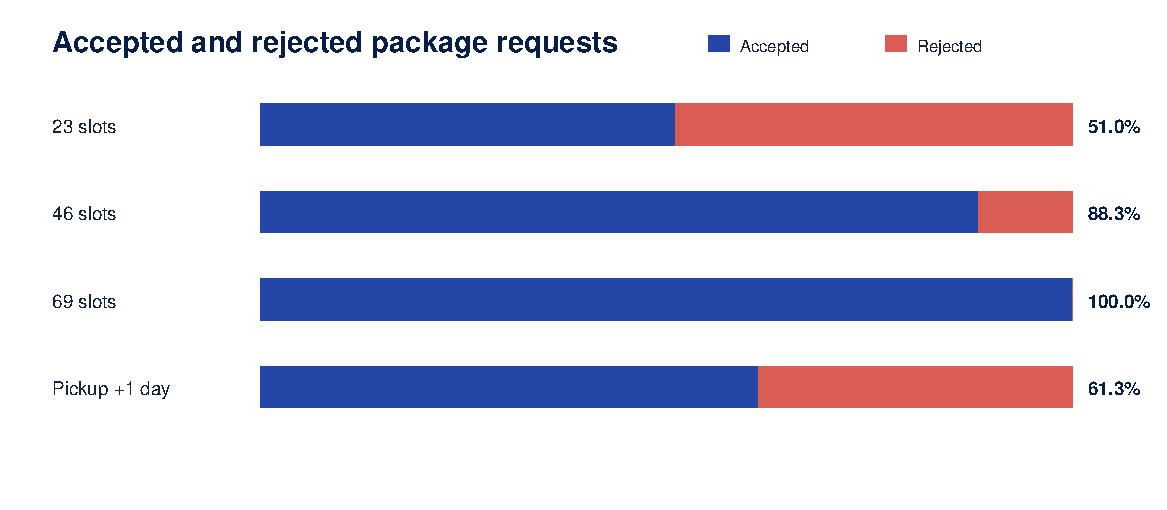
\includegraphics[width=0.78\linewidth]{scenario_comparison.pdf}\end{center}
\begin{center}\scriptsize\begin{tabular}{lrrr}
\toprule
\textbf{Scenario} & \textbf{Accepted} & \textbf{Rejected} & \textbf{Rate}\\
\midrule
23 slots per locker & 464 & 445 & 51.0\%\\
46 slots per locker & 803 & 106 & 88.3\%\\
69 slots per locker & 909 & 0 & 100.0\%\\
Pickup delayed by 1 day & 557 & 352 & 61.3\%\\
\bottomrule
\end{tabular}\end{center}
\vspace{1mm}\fcolorbox{amazonorange}{amazonorange}{\parbox{0.92\linewidth}{\scriptsize\color{navy}\textbf{Result:} 69 slots serve all 909 requests; a one-day pickup delay cuts acceptance by 246 packages. \textbf{Action:} reserve capacity jointly across days and treat faster pickup as a capacity lever.}}}



\end{poster}
\end{document}